%\chapter{Preliminaries}



\chapter{提案手法}

\section{従来手法との相違点}

従来手法では$L$を各物体の位置,トラジェクタ動作開始点,画面中央に限定しており,\ref{kadai}で述べた課題点を解決することができない.
その点を踏まえ,提案手法では複数の参照点を学習に利用する手法を導入した.従来手法の拡張で複数の参照点を考慮できるようにするためには,参照点と変位である座標系のいずれかに複数の参照点の情報を保持する機構を導入する必要がある.そこで参照点の候補に各参照点間の重心位置を採用する.また本研究では物体移動動作を初期状態に対する最終状態の決定と定義し,動作軌跡に関しては考慮しないため,学習モデルはより単純なガウスモデルを使用する.

\section{提案手法の概要}

\subsection{参照点}

従来手法で採用されていた各物体位置,トラジェクタの初期位置,画面中央に加えて,提案手法では新たに2つ以上の任意の物体間の重心位置を参照点に含める.すなわち環境中の$n$個の物体に対して,参照点は任意の物体間の重心を含めた$2^{n}+1$個を候補として考慮する.

\subsection{変位}

複数の物体間の相対的な位置関係を考慮する場合,座標系$k$の定め方として,参照点を原点とし,他の物体方向に軸を向けた座標系を考慮する必要があると考えられる.
そのため提案手法では,従来手法で採用されていた$k_{id}$,$k_{lt}$に,新たに1つの座標系を加えた以下の3種類が存在するとする.

\clearpage
 
	\begin{enumerate}
		\item 参照点を原点とし,常に一定の相対位置に遷移する
		\item 参照点を原点とし,トラジェクタの初期位置に応じて遷移先が変化する
		\item 複数の物体の位置関係に応じて遷移先が変化する
	\end{enumerate}
これら3種類の違いについてFig.\ref{figure:difference_displacement}で示す.
%%%%%%%%%%%%%%%%%%%%%%%%%%%%%%%%%%%%%%%%%%%%%%%%%%%%%%%%%%%%%%%%%%%%%%%%%%%%%%%%%%%%%%%%%%%%%%%%%%%%%%%
\begin{figure}[h]
	\centering
	\begin{minipage}[t]{.3\textwidth}
		\centering
		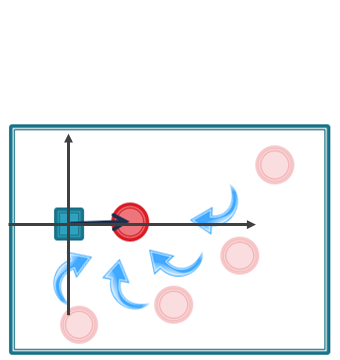
\includegraphics[width=4.7cm]{figure2_sub_a.png} \\ %TeXの基本として, \\ で緊急改行ができる.(今回の場合や行列などを除き,あまり使わない)
		\subcaption{トラジェクタ初期位置に対して一定}
		\label{subfigure:difference_displacement1}    
	\end{minipage}
	\begin{minipage}[t]{.3\textwidth}
		\centering
		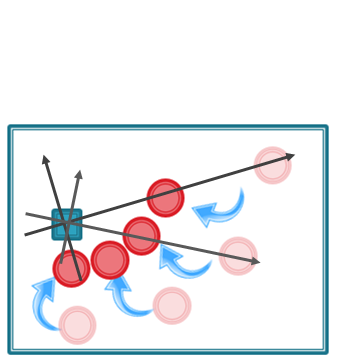
\includegraphics[width=4.7cm]{figure2_sub_b.png} \\ %TeXの基本として, \\ で緊急改行ができる.(今回の場合や行列などを除き,あまり使わない)
		\subcaption{空間上の特定の位置}
		\label{subfigure:difference_displacement2}
	\end{minipage}
	\begin{minipage}[t]{.3\textwidth}
		\centering
		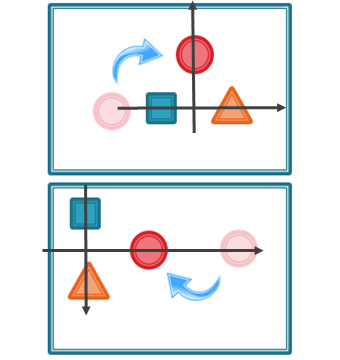
\includegraphics[width=4.7cm]{figure2_sub_c.png} \\ %TeXの基本として, \\ で緊急改行ができる.(今回の場合や行列などを除き,あまり使わない)
		\subcaption{他物体の位置に応じて変化}
		\label{subfigure:difference_displacement3}
	\end{minipage}
	\caption{参照点に対する遷移の違い}
	\label{figure:difference_displacement}
\end{figure}
%%%%%%%%%%%%%%%%%%%%%%%%%%%%%%%%%%%%%%%%%%%%%%%%%%%%%%%%%%%%%%%%%%%%%%%%%%%%%%%%%%%%%%%%%%%%%%%%%%%%%%%


Fig.\ref{subfigure:difference_displacement3}の例として,トラジェクタである丸い物体と参照点である三角の物体と四角い物体で,この順序で時計回りに正三角形を構成するよう並べる,という動作が考えられる.その動作においてトラジェクタの目標位置は2つの物体の相対的な位置関係によって決定されるが,図のように2つの物体の重心を参照点として座標系の原点とし,三角あるいは四角い物体の向きに軸をとった座標系$k_{gl}$において常に一定の位置を示す.
以下,本文中ではFig.\ref{subfigure:difference_displacement3}を重心-ランドマーク座標$k_{gl}$と定義する.

従って,推定すべき観点$<l , k>$は$2^{n}+1$個の参照点$l$のうち1つと3種類の座標系$k$のうち1つの対として表される.

\section{動作学習}

想定される観点の候補$<l , k>∈V$のそれぞれに,学習モデルとしてガウスモデルを設定し,その平均,2乗平均,標準偏差をそれぞれ$μ_{lk}$,$Q_{lk}$,$σ_{lk}$とする.
教示動作が与えられたとき,各観点のガウスモデルを以下のように更新する.

\begin{equation}
	v = Norm_{lk}(Trans_{lk}(p))
\end{equation}

\begin{equation}
	μ_{lk}  \leftarrow \frac{N}{N+1}μ_{lk}+\frac{1}{N+1}v
\end{equation}
\begin{equation}
	Q_{lk}  \leftarrow \frac{N}{N+1}Q_{lk}+\frac{1}{N+1}v^2	
\end{equation}
\begin{equation}
	σ_{lk}  \leftarrow \sqrt{Q_{lk} - μ_{lk}^2}
\end{equation}

ここで,$p$は教示動作の目標位置を指す.$Norm_{lk}$,$Trans_{lk}$はそれぞれその観点における正規化関数と座標変換を指し,以下の式で与えられる.

%まず教示動作の目標位置の,各参照点を原点とした相対位置を求め,各座標系ごとに座標変換,正規化を行う.それにより得たベクトル$v$を用いて,観点$<l , k>$のガウスモデルの平均$μ_{lk}$,2乗平均$Q_{lk}$,標準偏差$σ_{lk}$をそれぞれ更新する.
\begin{equation}
	Trans_{lk}(v) = 
	\begin{pmatrix}
        	\cos θ_{lkv} & \sin θ_{lkv} \\
        	-\sin θ_{lkv} & \cos θ_{lkv}
	\end{pmatrix}
	(v-Pos(l))
\end{equation}
\begin{equation}
	\label{equation:Norm}
	Norm_{lk}(v) = 
	\begin{cases}
		v & (if\,\,k=k_{id}) \\
		\frac{unit}{| Pos(r_{k})-Pos(l) |}v & (otherwise)
	\end{cases}
\end{equation}

ただし,$unit$は正規化長を表し,

\[
	\cos θ_{lkv} = \frac{(v-Pos(l))・(Pos(r_{k})-Pos(l))}{| v-Pos(l) || Pos(r_{k})-Pos(l) |}
\]

であり,$Pos(l)$は参照点$l$の位置ベクトルを表す.また$r_{k}$は座標系$k$が軸を向ける方向を決定する参照点を表す.例えば座標系$k_{lt}$の場合,$r_{k_{lt}}$はトラジェクタの初期位置を表す.
正規化関数の必要性と性質については\ref{subsection:UNIT}で述べる.

\section{動作再現}

教示動作から学習された各観点$<l , k>$における確率モデルを用いて,トラジェクタの目標位置$v$を以下のように求めることで,学習動作の再現を行う.
\begin{equation}
	v =  Pos(\hat{l}) +Trans^{-1}(Norm^{-1}(μ_{\hat{l}\hat{k}})) 
\end{equation}
\begin{equation}
	<\hat{l} , \hat{k}> =  \mathop{\arg\min}_{k , l}σ_{lk}
\end{equation}

まず学習された各観点のガウスモデルのうち,最も分散の小さいものを探索する.分散が小さいとは教示動作がその観点に対して常に類似した目標位置に遷移していたことを意味し,教示者が意図した観点である可能性が高いと考えられるためである.選択された観点のガウスモデルの平均を,その観点と再現時の初期環境に応じた正規化と座標変換の逆関数を計算し,初期環境における参照点の位置に平行移動することで再現動作のトラジェクタの目標位置を推定する.
Fig.\ref{figure:learning_and_reproduction_model}に,提案手法における動作学習と動作再現の模式図を示す.
%%%%%%%%%%%%%%%%%%%%%%%%%%%%%%%%%%%%%%%%%%%%%%%%%%%%%%%%%%%%%%%%%%%%%%%%%%%%%%%%%%%%%%%%%%%%%%%%%%%%%%%
	\begin{figure}[h]
%中央ぞろえ
		\begin{center}
			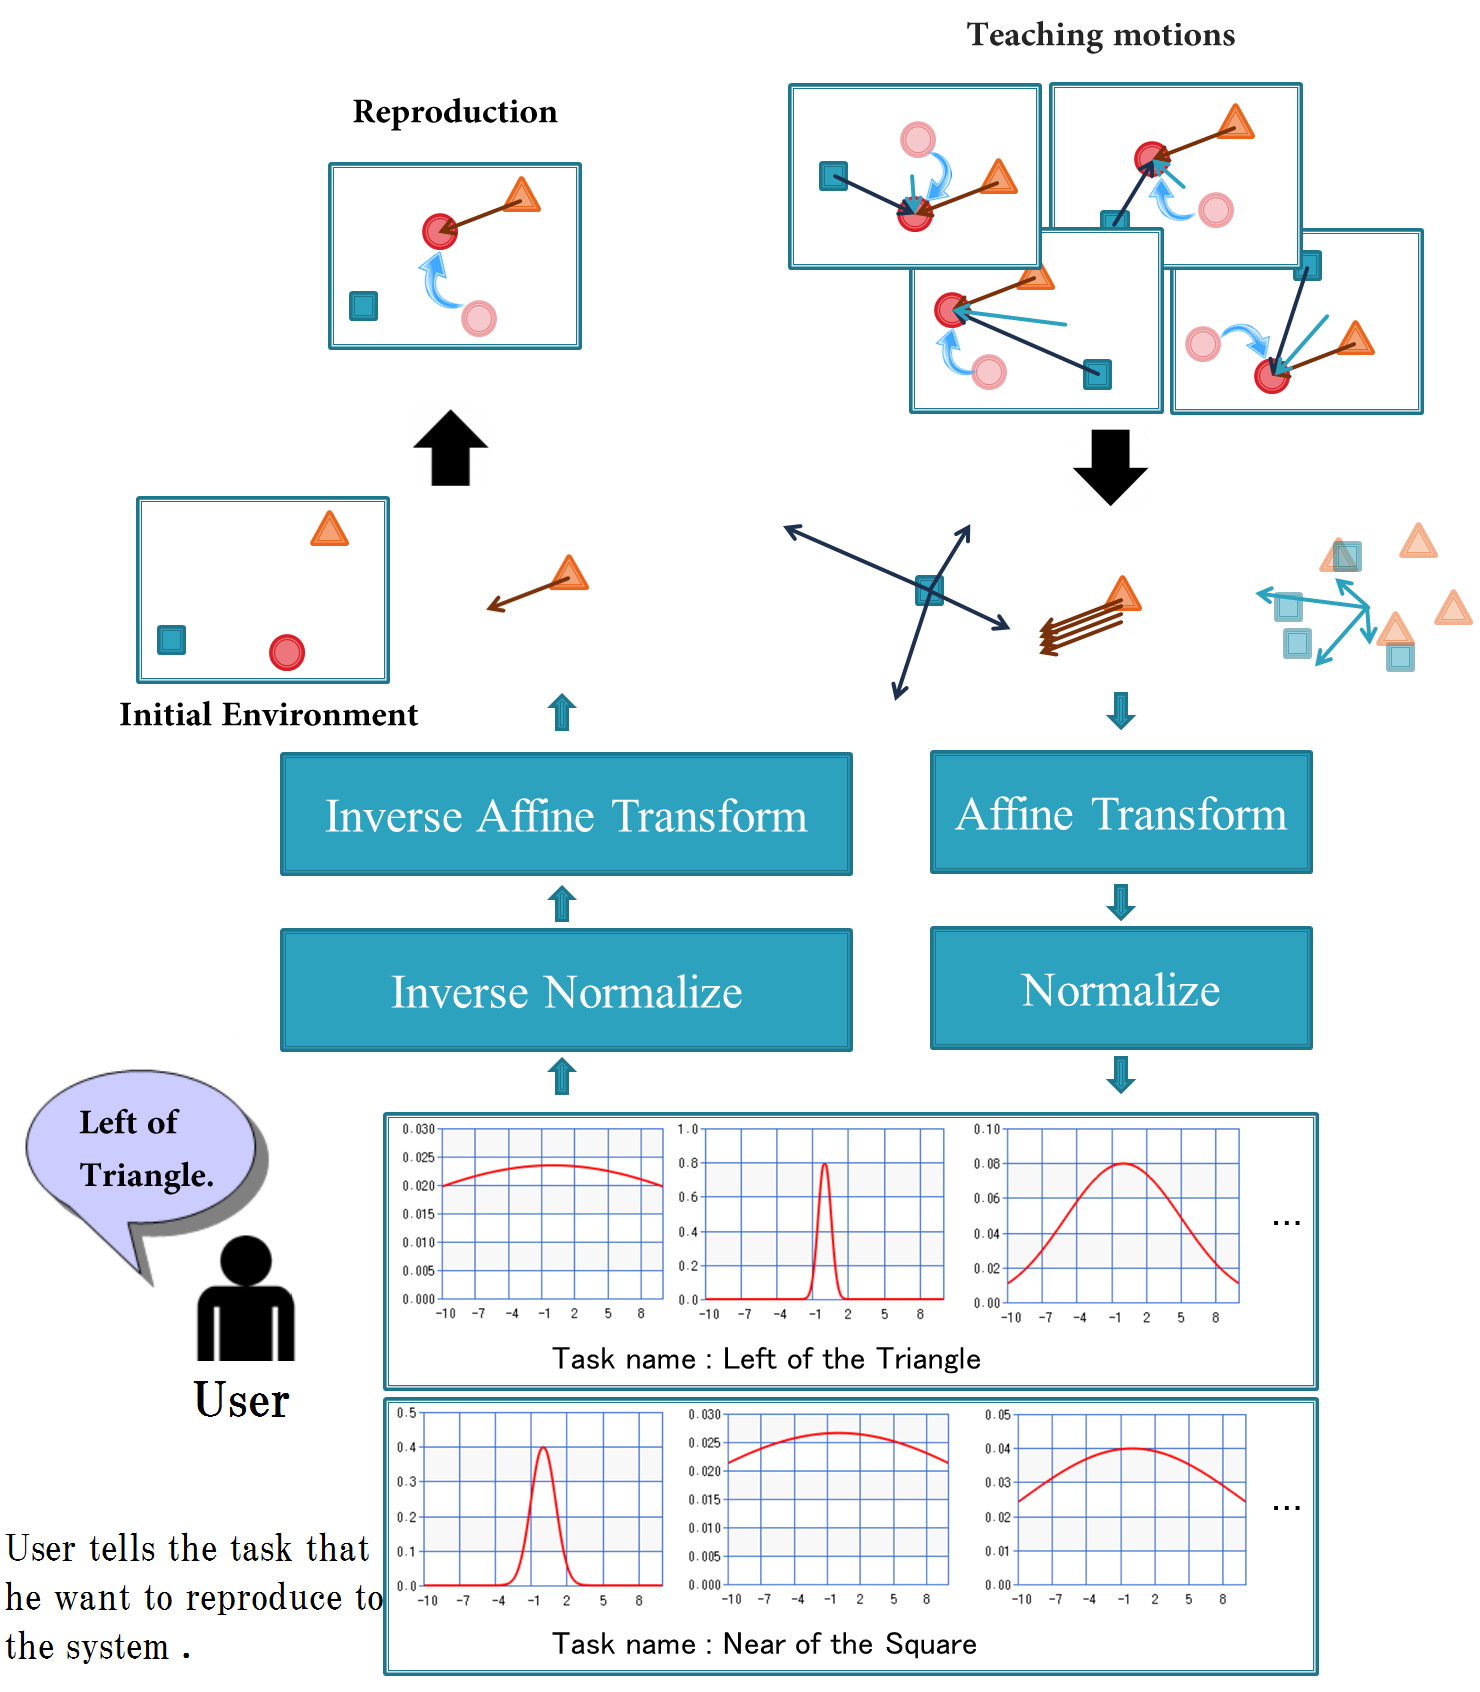
\includegraphics[width=12cm]{chart9.png} \\ %Teの基本として, \\ で緊急改行ができる.(今回の場合や行列などを除き,あまり使わない)
			\caption{動作学習と動作再現}
			\label{figure:learning_and_reproduction_model}
		\end{center}
	\end{figure}
%%%%%%%%%%%%%%%%%%%%%%%%%%%%%%%%%%%%%%%%%%%%%%%%%%%%%%%%%%%%%%%%%%%%%%%%%%%%%%%%%%%%%%%%%%%%%%%%%%%%%%%

\section{動作識別}

動作ごとに学習された観点集合$V_{t}$を用いて,目標位置が$p$である例示動作の属する動作$t∈T$を以下のように推定することで,例示動作の識別を行う.

\begin{equation}
	\label{equation:identification function}
	t =  \mathop{\arg\max}_{t}Probability(<l , k>∈V_{t} , p)
\end{equation}

\begin{equation}
	\label{equation:generation probability}
	Probability(<l , k> , p) = \frac{1}{\sqrt{2\pi}σ_{lk}}\exp \left(\frac{|Norm_{lk}(Trans_{lk}(p))-μ_{lk}|^2}{2σ_{lk}^2}\right)
\end{equation}

ここで$T$は既学習動作の集合を表し,$V_{t}$とは動作$t$を学習した観点の学習モデルの集合を表す.
まず各動作において学習されたガウスモデルから,$p$が生起される確率である\ref{equation:generation probability}式をそれぞれ求め,生起確率が最大となるガウスモデルを持つ動作を識別結果とする.また,\ref{equation:identification function}式に閾値を設定し,以下のように定義し直すことで,未学習動作の推定が可能になる.

\begin{equation}
	\label{equation:identification function2}
	t =
	\begin{cases}
		\mathop{\arg\max}_{t}Probability(V_{t} , p)		& (\mathop{\max}_{t}Probability(V_{t} , p) > Threshold) \\
		t_{unknown}					 			& (otherwise)
	\end{cases}	
\end{equation}
ここで,$t_{unknown}$は未学習動作を表す.
